\documentclass[a4paper,12pt]{scrartcl} 
\usepackage{ulem}
\usepackage{graphicx}
\usepackage{amsmath}
\usepackage[warn]{mathtext} 
\usepackage[T2A]{fontenc} 
\usepackage[utf8]{inputenc}
\usepackage[english]{babel} 
\usepackage{indentfirst} 
\usepackage{misccorr} 
\usepackage{caption}
\usepackage{graphicx}
\usepackage{subcaption}
\usepackage{xcolor}
\usepackage{wrapfig}
\usepackage{algorithm}
\usepackage{algpseudocode}
\captionsetup{compatibility=false}
\begin{document}

\title{SyntenyFinder: A Synteny Blocks Generation and Genome Comparison Tool}
\author{Intern: Ilya Minkin\\
	Advisor: Son Pham}
\date{}
\maketitle

\begin{abstract}
We present an algorithm for finding synteny blocks in genomes. The algorithm is based on colored de Bruijn graphs and graph simplifications.
Our method is suitable for finding synteny blocks in genomes that contain regions of highly conserved DNA, i.e. genomes that are evolutionary
close to each other. With some modifications the algorithm can be applied in more complicated cases.
\end{abstract}

\section{Introduction}

Recent advances in high throughput sequencing and genome assembling technologies result in appearance of high number of
completely sequenced genomes, ranging from bacteria to mammalian \cite{Genome10K}. It raises a lot of interesting 
biological question. For example, it is not obvious how DNA sequence leads to observable phenotype. Comparative genomics
addresses this question using the fact that common features of two organisms are often encoded by DNA regions that are conserved
within the species \cite{ComparativeGenomics}. 

Another question is evolution. It is known that genome rearrangements play important role in adaptation in adaptation of bacteria
for different environments \cite{GenomeEvolutionAdaptation}. And the more exciting is study of mammalian evolution \cite{HumanMouse}.

In order to perform rearrangement analysis, the genomes must be decomposed into conservative segments,
called synteny blocks. Currently existing tools for solving this problem, like DRIMM-Synteny
\cite{Pham2010}, require the genomes to be presented as sequences of enumerated local alignments, or \textit{anchors}.

De Bruijn graphs are extensively used in bioinformatics for genome assembly \cite{Pevzner2001, Iqbal2012}. 
In this work we address problem of finding synteny blocks from nucleotide sequences. We propose new 
algorithm for this task based on colored de Bruijn graph.

\section{Problem definition}

Suppose that we are given a set \(S = \lbrace S_{1}, S_{2}, \ldots, S_{n} \rbrace \) of chromosomes, and each
chromosome is represented as a string over alphabet \(\lbrace A, C, G, T \rbrace \). The task of finding synteny
blocks is to find a set of so called conserved regions \(C = \lbrace C_{1}, C_{2}, \ldots , C_{n} \rbrace \), where
each conserved region \(C_{i}\) is a set of substrings of chromosomes from \(S\). Such regions are supposed 
to cover most of the genome for closely related species.  All substrings forming a conserved region \(C_{i}\) must be
similar to each other according to some criterion of similarity. Note that problem of finding synteny blocks in a set
of chromosomes is equivalent to a problem of finding synteny blocks in one superchromosome
obtained from concatenating all chromosomes from the set -- we can just separate chromosomes by special characters.

At this moment there is no generally accepted formal criterion of similarity exist, so the problem of finding synteny blocks is ill-defined.
In our work we introduce new criterion of similarity based on de Bruijn graphs and graph simplifications.

\section{General idea}

\begin{figure}
        \begin{subfigure}[a]{1\textwidth}
		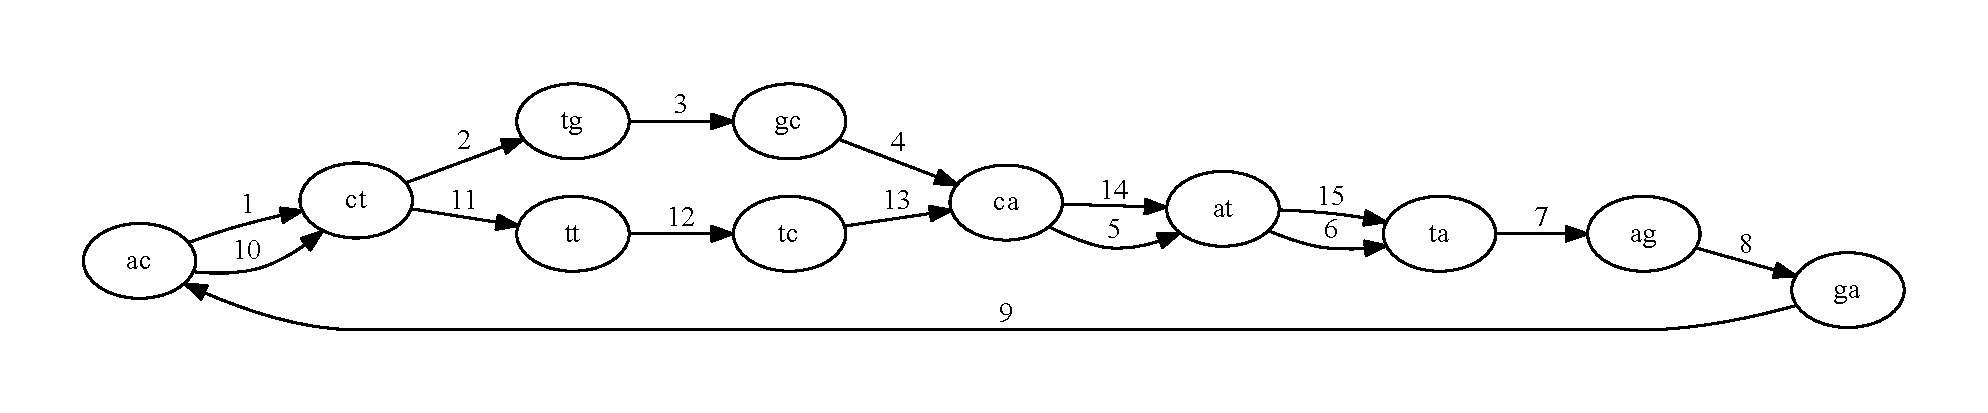
\includegraphics[scale = 0.50]{graph1.pdf}
		\small \caption{De Bruijn graph built from string \("acgcattgtactcatt"\) and \(k = 2\). Non-branching paths correspond to multiple
			copies of the same substrings.}
		\label{DeBruijnA}
        \end{subfigure}
	\\
        \begin{subfigure}[b]{1\textwidth}
		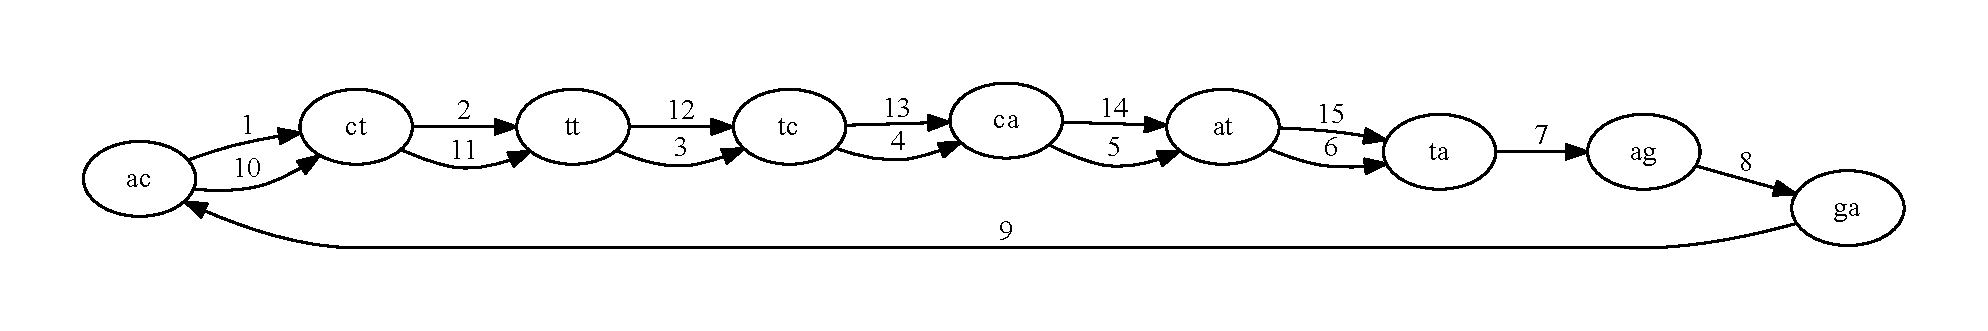
\includegraphics[scale = 0.50]{graph2.pdf}
		\small \caption{Same de Bruijn graph after simplification. Replacing \("acGca"\) by \("acTca"\) we obtain long non-branching path
			that corresponds to the synteny block.}
		\label{DeBruijnB}
        \end{subfigure}
	\small \caption{Illustration of de Bruijn graphs and graph simplification}
\end{figure}

As previously mentioned, our method is based on de Bruijn graph.
Given a fixed value \(k\) and a string \(S\) we can build de Bruijn graph \(G\) from the string as follows.
Let's denote by \(k\)-prefix of a string \(S\) first \(k\) characters of \(S\), and by \(k\)-suffix last \(k\) characters of \(S\).
For each unique substring of length \(k\) (called \(k\)-mer) found in \(S\), we add a vertex to \(G\) and mark it with
corresponding \(k\)-mer. For each \((k + 1)\)-mer \(w\) found in \(S\) we add edge that connects vertex corresponding to
\(k\) prefix of \(w\) with vertex corresponding to \(k\) suffix of \(w\) and label the edge with position of first character of \(w\)
(multiedges with different labels are allowed).

In this graph we consider only paths that have consecutive labels on edges. It is easy to see that with such restriction every path in \(G\)
corresponds to a substring in \(S\). Example of such de Bruijn graph built from the string \(S = "acgcattgtactcatt" \) and \(k = 2\) is
depicted on Figure~\ref{DeBruijnA}.

Note that two copies of substring \("catt"\) form a non-branching path consisting of edges with multiplicity \(2\) in this graph. Single
mismatch in substrings \("acGca"\) and \("acTca"\) form so-called "bulge", unoriented cycle generated by two valid paths with
coinciding ends. If we replace one branch of the bulge by another (replace \("acGca"\) by \("acTca"\) for example), we will obtain
a long non-branching path (Figure~\ref{DeBruijnB}).

This heuristic forms basis of our method -- conserved regions in different parts of the genome contain conserved basepairs, but
such regions are disrupted by indels and mismatches. These differences form bulges in the graph that make it different to infer
structure of the synteny blocks. We remove bulges having size less than some predefined constant and thus obtain non-branching
paths corresponding to the conserved regions. The process of removing bulges from the graph is called \textit{simplification}. We
sustain one-to-one correspondence between the graph and the string -- when we change something in the graph, then we change
appropriate characters in the string.

Conserved regions can be located on opposite strands of DNA. To handle this, we use \textit{colored} de Bruijn graphs \cite{Iqbal2012}.
Given a string \(S\), for each \((k + 1)\)-mer found in \(S\) we add corresponding edge to the graph and color it \textit{blue}, for 
each \((k + 1)\)-mer found in reverse-complementary counterpart of \(S\) we add corresponding edge to the graph and color it \textit{red}.
In this graph, non-branching paths with different colors represent synteny blocks located on opposite strands of DNA.

Complete pipeline is following:\\
1) Concatenate input chromosomes into one superchromosome \\
2) Build de Bruijn graph from the superchromosome \\
3) Simplify the graph \\
4) Output synteny blocks as non-branching path in the graph 

Our algorithm depends on two parameters: \(k\) and \(\delta\) (minimum allowed size of a bulge). It is reasonable to use as high \(k\) as possible
\((k > 50)\) to keep graph structure simple and avoid connecting regions that are actually not homologous. So, our method requires that conserved regions
in input genomes contain exact shared \(k\)-mers. This is not a problem in genomes that are very close to each other (like different strains of a bacteria),
but it can create difficulties in genomes that had separated a long time ago.

This issue can be solved, for example, by finding a set of all local alignments in the genomes and substituting one subsequence in each found alignment
by another. In results section we will demonstrate on a practical half-synthetic example that with such modifications our method is able to handle
complicated cases. So at this point our method is directly applicable to only evolutionary close genomes and  in near future we plan to extend it to
wider range of use.

\section{Detailed description}

In this section we formally describe our algorithm for finding synteny blocks. We are given two numbers \(k\) and \(\delta\) and a
set \(S = \lbrace S_{1}, S_{2}, \ldots, S_{n} \rbrace \) of chromosomes,
where each chromosome  \(S_{i} = (s_{i, 1}, s_{i, 1}, \ldots, s_{i, m_i})\) is a string over alphabet \(\Sigma = \lbrace A, C, G, T \rbrace\).
Let's denote by \(X_{1} \uplus X_{2}\) concatenation of strings \(X_{1}\) and \(X_{2}\). We denote by \(X[i, j]\) a substring of a string \(X\) that
starts at \(i\) and ends at \(j\), \(X[i, j] = (x_{i}, x_{i + 1}, \ldots, x_{j}) \). \(Rev(X)\) means reverse-complementary counterpart of a string \(X\).

First step of the algorithm is to obtain superchromosome \(\hat{S} = S_{1} \uplus S_{2} \uplus \ldots \uplus S_{n} \). Concatenated
strings are interleaved by special characters that indicate ends of the chromosomes, but we omit these technical details. Then we build a linked list of
pairs \(L = ((\hat{s}_1, 1), (\hat{s}_2, 2), \ldots, (\hat{s}_{m}, m))\) and \(l_i\) is a pointer to \(i\)-th item in the list, \(Next(l_i) = l_{i + 1}\) is next
element after \(l_i\). Let's denote by \(l_i[1]\) first element of pair of \(i\)-th item of the list (\(l_i[2]\) is second element). First element of a pair represents
character of the sequence, and second element represents it's original position in string \(\hat{S}\). 

Colored de Bruijn graph is graph \(G = (V, E) \) where \(V = \Sigma ^ k \). Set of outgoing edges from vertex \(v\) is denoted \(Out(v)\). We define three functions: \\
1) \(Pos : \, E \rightarrow \lbrace l_1, l_2, \ldots , l_m \rbrace \) \\
2) \(Color : \, E \rightarrow \lbrace Blue, Red \rbrace \) \\
3) \(Spell: \, E \rightarrow \Sigma ^ {k + 1} \)

For each \(i \in \lbrace{1, 2, \ldots, n - k} \rbrace \) we add two oriented edges to the graph: \\
1) \(e^+ = (\hat{S}[i, i + k - 1], \hat{S}[i + 1, i + k]) \), where: \\
\(Color(e^+) = Blue, \,  Pos(e^+) = l_i, \, Spell(e^+) = \hat{S}[i, i + k] \) \\
2) \(e^- = (Rev(\hat{S}[i, i + k - 1]), Rev(\hat{S}[i + 1, i + k]))\), where: \\
 \(Color(e^-) = Red, \, Pos(e^-) = l_{i + k - 1}, \, Spell(e^-) = Rev(\hat{S}[i, i + k])\)

A \textit{valid} path in \(G\) is a sequence of edges \(P = (e_{1}, e_{2}, \ldots, e_{n})\) iff \(Pos(e_{i+1})  = Next(Pos(e_{i}))\) and
\(Color(e_{i + 1}) = Color(e_{i})\). Let's denote by \(Start(P)\) first vertex of the path \(P\) and by \(End(P)\) the last vertex of \(P\).

\newpage

A pair of valid paths \(B =\lbrace b_{1}, b_{2} \rbrace \)
is called a \textit{bulge}, iff following holds: \\
1) \(Start(b_{1}) = Start(b_{2}) \wedge End(b_{1}) = End(b_{2}) \) \\
2) \(b_{1}\) and \(b_{2}\) have no common vertices except \(Start(b_{1})\) and \(End(b_{1})\) \\
3) There are no edges \(e_{1} \in b_{1}, e_{2} \in b_{2} \) such that \(Spell(e_{1}) = Spell(e_{2})\) \\
4) Their sets of positions do not intersect (I'll define it a bit later) 

A bulge \(B =\lbrace b_{1}, b_{2} \rbrace \) is called \textit{bad} iff \(|b_1| < \delta \wedge |b_2| < \delta\) where \(\delta\) is a parameter.

A vertex \(v\) is called \textit{bifurcation} iff there are at least two outgoing (ingoing) edges \(e_{1}, e_{2}\) 
incident \(v\) such that \(Spell(e_{1}) \neq Spell(e_{2})\). A set of paths \(P_{nb} = \lbrace P_{1}, P_{2}, \ldots, P_{n} \rbrace\)
is said to form a \textit{non-branching path} iff \(|P_{1}| = |P_{2}| = \ldots |P_{n}| \) and \(Spell(e_{i, k}) = Spell(e_{j, k}) \),
where \(e_{i, j}\) denote \(j\)-th edge in the \(i\)-th path, i.e. all paths spell the same substring.

\begin{figure}
	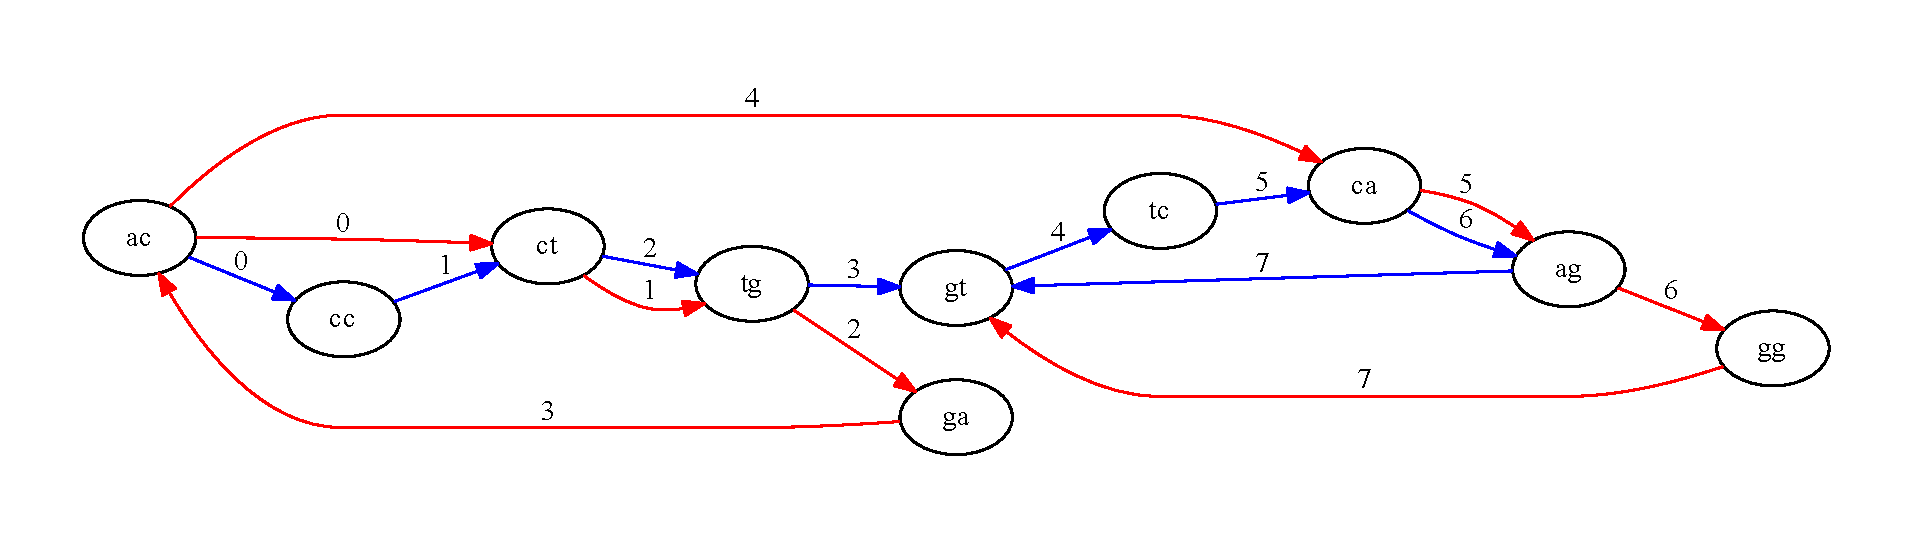
\includegraphics[scale = 0.50]{graph3.pdf}
	\small \caption{Colored de Bruijn graph for string \(S = "acctgtcagt" \) }
	\label{ColoredDeBruijn}
\end{figure}

Let's illustrate above definitions on a simple example. Colored de Bruijn graph built from string \(\hat{S} = "acctgtcagt"\)
is depicted on figure~\ref{ColoredDeBruijn}. Here \(Rev(\hat{S}) = "actgacaggt"\). Edges' labels denote indices of elements of
list \(L\). Vertices \("ac", "ct", "tg"\) are bifurcations, while \("cc", "tc", "ga"\) are not. Two paths \(("ac", "ct")\) and \((("ac", "cc"), ("cc", "ct"))\)
form a bulge. Two multiedges \(("ct", "tg")\) form a non-branching path.

Pseudocode of our algorithm for synteny blocks finding is below. Actually, it lacks some important details, so I will augment it later.

\begin{algorithm}[H]               
\small \caption*{\(SyntenyFinder(S = \lbrace S_{1}, S_{2}, \ldots, S_{n} \rbrace,  k, \delta)\)} 
\label{Pseudocode}
\begin{algorithmic}[1]     
\State \(\hat{S} = S_{1} \uplus S_{2} \uplus \ldots \uplus S_{n} \)
\State \(L = ((\hat{s}_1, 1), (\hat{s}_2, 2), \ldots, (\hat{s}_{m}, m))\)
\State \(G = BuildDeBruijn(L, k)\)
\State \(run = True\)
\While{\(run == True\)}
	\State \(run = False\)
	\For{\(v \in V(G)\)}
		\For{\(e_1, e_2 \in Out(v)\)}
			\If{\(FormBadBulge(e_1, e_2,  \delta)\)}
				\State \(run = True\)
				\State \(ReplaceBranch(e_1, e_2)\)
			\EndIf
		\EndFor
	\EndFor
\EndWhile
\State \(OutputNonBranchingPaths(G)\)
\end{algorithmic}
\end{algorithm}

\section{Experimental results}
Results
\section{Conclusion}
Conclusion

\begin{thebibliography}{9}
\bibitem{Genome10K}
	Genome 10K Community of scientists.
	Genome 10K: A proposal to obtain whole-genome sequence for 10000 vertebrate species.
	Journal of Heredity, 100(6): 659-674.
\bibitem{ComparativeGenomics}
	Ross C. Hardison.
	Comparative genomics.
	PLoS Biology 1(2): e58.
\bibitem{GenomeEvolutionAdaptation}
	Fabien Aujoulat, Frederic Roger, Alice Bourdier, Anne Lotthe  Brigitte Lamy, Helene Marchandin, Estelle Jumas-Bilak.
	From environment to man: genome evolution and adaptation of human opportunistic bacterial pathogens.
	Genes 2012, 3(2), 191-232.
\bibitem{HumanMouse}
	Pavel Pevzner, Glenn Tesler.
	Genome rearrangements in mammalian evolution: lessons from human and mouse genomes.
	Genome Research. 2003 Jan;13(1):37-45.
\bibitem{Kellis2004}
	Manolis Kellis, Bruce W. Birren, Eric S. Lander.
	Proof and evolutionary analysis of ancient genome duplication in the yeast Saccharomyces cerevisiae.
	Nature 2004 Apr 8;428 (6983): 617-24.
\bibitem{Pham2010}
	Son K. Pham, Pavel A. Pevzner.
	DRIMM-Synteny: decomposing genomes into evolutionary conserved segments.
	Bioinformatics (2010)  26  (20):  2509-2516.
\bibitem{Pevzner2001}
	Pavel A. Pevzner, Haixu Tang, Michael S. Waterman.
	An Eulerian path approach to DNA fragment assembly.
	Proc. Natl. Acad. Sci. USA. 2001 Aug 14; 98(17): 9748-53.
\bibitem{Iqbal2012}	
	Zamin Iqbal, Mario Caccamo, Isaac Turner, Paul Flicek, McVean.
	De novo assembly and genotyping of variants using colored de Bruijn graphs.
	Nat Genet. 2012 Jan 8;44(2):226-32. doi: 10.1038/ng.1028.
\end{thebibliography}

\end{document}